% !TeX spellcheck = en_UK

\documentclass[10pt]{beamer}
\usepackage{mystyle}

%\includeonly{}
\begin{document}

\section{Reeb graph}

\subsection{Definition}
\begin{frame*}
Given:
\begin{itemize}
\item<1-> a manifold $\mathcal{M}$;
\item<2-> a Morse function $\map{f}{\mathcal{M}}{\RR}$ with distinct critical values;
\end{itemize}
\onslide<3->{
the \defterm{Reeb graph} of $f$ is the $1$-dimensional simplicial complex
\[
\mathcal{R}(f)=\mathcal{M}/\sidenote<4>[text height=height("I"))]{\sim}{\draw node[draw,circle,inner sep=5pt] (source)  {} node[text width=4cm,anchor=north west] (target) at (.3,-.3) {$x\sim y$ if $f(x)=f(y)$ and they belong to the same connected component of $f^{-1}(f(x))$} (source) to[out=-90,in=170] ([yshift=-7pt]target.north west);}.
\]
}
\onslide<5->{
The \defterm{segmentation map} is the quotient map
\[
\map{\Phi}{\mathcal{M}}{\mathcal{R}(f)}.
\]
}
\vspace{-.9cm}
\begin{center}
\tikzexternalenable
\begin{tikzpicture}
\colorlet{topcolor}{gray!40!white!30!red}
\colorlet{bottomcolor}{gray!40!white!30!blue}
\def\preimageh{19.1}
\tikzmath{\hpercent=int(\preimageh/25*100);}
\colorlet{preimagecol}{topcolor!\hpercent!bottomcolor}
\path (-2,-.1) rectangle (6.5,3.3);
\begin{scope}[small,transform canvas={scale=.5}]
\begin{onlyenv}<2->
\begin{scope}[shift={(-12,0)}]
\draw[black,line width=2pt] (-1.5pt,0) rectangle (1.5pt,25);
\path[decorate,decoration={markings,mark=at position 1 with{\arrow{Latex[line width=1pt,fill=topcolor,scale=3]};}}] (0,0) to node[left,scale=2] {$f$} ($(0,25)+(0,13pt)$);
\fill[top color=topcolor,bottom color=bottomcolor] (-1.5pt,0) rectangle (1.5pt,25);
\scoped[shift={(0,\preimageh)}]\draw[/visible on=<4>,line width=1pt,fill=preimagecol] coordinate (level set l) (-4pt,-4pt) rectangle (4pt,4pt);
\end{scope}
\end{onlyenv}
\draw[/visible on=<5>,line width=1pt,-{To}] (20,12.5) -- node[above,scale=2] {$\Phi$} (27,12.5);
\alt<2>{\pic{reeb graph={manifold 1,contour,background={\fill[top color=topcolor,bottom color=bottomcolor] (bbox.south west) rectangle (bbox.north east);}}};}
{\pic{reeb graph={manifold 1,manifold bg,/only=<4>{
partial edge={12}{}{absolute slice={\preimageh}{slice}{\pic[preimagecol,line width=2pt]{slice circle 2=.12cm between (slice-2) and (slice-1)};}},
partial edge={11}{}{absolute slice={\preimageh}{slice}{\pic[preimagecol,line width=2pt]{slice circle 2=.12cm between (slice-2) and (slice-1)};}},
partial edge={10}{}{absolute slice={\preimageh}{slice}{\pic[preimagecol,line width=2pt]{slice circle 2=.12cm between (slice-2) and (slice-1)};}},
},/only=<5>{every segment={\fillsegmentcmd}}}};}
\begin{scope}[xshift=8cm]
\begin{onlyenv}<3->
\pic{reeb graph={manifold 1,every edge={preaction={draw=black,line width=3pt},/alt=<5>{draw=\thiscolor}{draw=gray!40},line width=2pt},every node={\draw[black,line width=1pt,fill=white] circle(3pt);},/only=<4>{
partial edge={12}{}{absolute up to={\preimageh}{\fill[preimagecol] circle(3pt);}},
partial edge={11}{}{absolute up to={\preimageh}{\fill[preimagecol] circle(3pt);}},
partial edge={10}{}{absolute up to={\preimageh}{\fill[preimagecol] coordinate (level set r) circle(3pt);}},}
}};
\end{onlyenv}
\end{scope}
\only<4>{\scoped[on background layer={transform canvas={scale=.5}}]\draw[line width=1,preimagecol,dashed] (level set l) -- (level set r);}
\end{scope}
\end{tikzpicture}
\tikzexternaldisable
\end{center}
\end{frame*}

\subsection*{Desired algorithm}
\begin{frame*}
\begin{columns}[T,onlytextwidth]
\begin{column}{.7\textwidth}
\textbf{Input:}
\begin{itemize}
\item {\only<2->{\color{gray}}a PL manifold $\mathcal{M}$}\\
\onslide<2->{$\leadsto$ a triangulated mesh $\mathcal{M}$;}
\item<3-> {\only<4->{\color{gray}}a non-degenerate PL scalar field $f$ on $\mathcal{M}$}\\
\onslide<4->{$\leadsto$ a \sidenotehighlight<4>{scalar value}{\draw node[anchor=north west,text width=4cm] (target) at (.5, -.3) {pairwise different, in order to ensure non-degeneracy; this can be achieved by random perturbations} (mymark) to[out=-90,in=170] ([yshift=-7pt]target.north west);} $f(v)$ for each vertex $v$ of $\mathcal{M}$.}
\end{itemize}
\vspace{.4cm}
\onslide<5->{
\textbf{Output:}
\begin{itemize}
\item the \sidenotehighlight<5>{augmented}{\draw node[anchor=north west] (target) at (.5,-.3) {graph $+$ segmentation map} (mymark) to[out=-90,in=170] ([yshift=-7pt]target.north west);} Reeb graph $\mathcal{R}(f)$.
\end{itemize}
}
\end{column}
\begin{column}{.3\textwidth}
\tikzexternalenable
\begin{tikzpicture}
\colorlet{topcolor}{gray!40!white!30!red}
\colorlet{bottomcolor}{gray!40!white!30!blue}
\path(0,0) rectangle(3,3.5);
\begin{scope}[small,transform canvas={scale=.5},shift={(6,1)}]
\only<1-2>{\pic{reeb graph={manifold 1,manifold bg}};}
\only<3-4>{\pic{reeb graph={manifold 1,contour,background={\fill[top color=topcolor,bottom color=bottomcolor] (bbox.south west) rectangle (bbox.north east);}}};}
\only<5->{\pic{reeb graph={manifold 1,contour, every segment={\fillsegmentcmd},every edge={preaction={draw=white,line width=3pt},draw=\thiscolor,line width=2pt},every node={\draw[black,line width=1pt,fill=white] circle(3pt);}}};}
\end{scope}
\end{tikzpicture}
\tikzexternaldisable
\end{column}
\end{columns}
\vspace{.4cm}
\onslide<6->{
\textbf{Time complexity:}
\begin{itemize}
\item $O(m\cdot\log m)$, where $m$ is the \sidenotehighlight<6>{size}{\draw node[anchor=north east] (target) at (-.5,-.3) {$\#\text{vertices}+\#\text{edges}+\#\text{triangles}$} (mymark) to[out=-90,in=10] ([yshift=-7pt]target.north east);} of the $2$-skeleton of $\mathcal{M}$.
\end{itemize}
}
\vspace{.4cm}
\onslide<7->{
\textbf{Parallel.}
}
\end{frame*}

\subsection{Geometry of critical points}
\begin{frame*}
There are three kinds of critical points:
\begin{columns}[T,onlytextwidth]
\begin{column}{.55\textwidth}
\begin{itemize}
\item<2-> \textcolor{gray}{(local)} \textbf{maxima}\\
\onslide<9->{$\leadsto$ ${\color{orange}\Link^+}$ empty;}
\item<3-> \textcolor{gray}{(local)} \textbf{minima}\\
\onslide<10->{$\leadsto$ ${\color{violet}\Link^-}$ empty;}
\item<4-> \textbf{saddles}\\
\onslide<11->{$\leadsto$ ${\color{orange}\Link^+}$ or ${\color{violet}\Link^-}$ disconnected.}
\end{itemize}
\end{column}
\begin{column}{.45\textwidth}
\tikzexternalenable
\begin{tikzpicture}
\matrix[cells={scale=.5},row sep=7, row 1/.style={/visible on=<2->},row 2/.style={/visible on=<3->},row 3/.style={/visible on=<4->}]{
\draw[fill=gray!40] (-1,-1) arc(180:0:1) arc(0:-180:1 and .25);
\draw[postaction={/visible on=<10->,draw=violet,line width=1},dashed,opacity=.5,/visible on=<2->] (-1,-1) arc(180:0:1 and .25);
\draw[/visible on=<9->,violet,line width=1] (-1,-1) arc(-180:0:1 and .25);
\draw[fill=white] circle(3pt);\\
\draw[fill=gray!40] (-1,1) arc(-180:0:1) -- cycle;
\draw[postaction={/visible on=<10->,draw=orange,line width=1},fill=gray] (0,1) circle(1 and .25);
\draw[fill=white] circle(3pt);\\
\fill[gray] (-1,.4) arc(90:0:.6 and .3) arc(-180:0:.4 and .1) arc(180:90:.6 and .3) -- (1,0) to[bend left] (-1,0) -- cycle;
\fill[gray!40] (-1,-1) to[bend left] (1,-1) -- (1,-.2) arc(-90:-180:.6 and .3) arc(0:-180:.4 and .1) arc(0:-90:.6 and .3) -- cycle;
\draw[postaction={/visible on=<11->,draw=violet,line width=1}] (-1,-1) to[bend left] (1,-1);
\path[name path=first] (-1,0) to[bend right] (1,0);
\draw[name path=second,postaction={/visible on=<11->,draw=orange,line width=1}] (-1,-.2) arc(-90:90:.6 and .3) (1,-.2) arc(270:90:.6 and .3);
\draw[postaction={/visible on=<11->,draw=violet,line width=1},dashed,opacity=.5,/visible on=<4->,intersection segments={of={first and second}, sequence={L2}}];
\draw[postaction={/visible on=<11->,draw=violet,line width=1},intersection segments={of={first and second}, sequence={L1 L3}}];
\draw (-.4,.1) arc (-180:0:.4 and .1);
\draw[fill=white] circle(3pt);\\
};
\end{tikzpicture}
\tikzexternaldisable
\end{column}
\end{columns}
\onslide<5->{
\begin{block}{How to detect them on a PL manifold?}
\begin{columns}[T,onlytextwidth]
\begin{column}{.65\textwidth}
\onslide<6->{Given a vertex $v$, the {\color{blue!40}\defterm{star}} of $v$ is the union of all simplices containing $v$.\\}
\onslide<7->{The {\color{blue}\defterm{link}} of $v$ is the boundary of its star.}
\onslide<8->{
\begin{align*}
{\color{orange}\Link^+}(v)&=\left\{x\in\Link(v):f(x)>f(v)\right\}\\
{\color{violet}\Link^-}(v)&=\left\{x\in\Link(v):f(x)<f(v)\right\}\\
\end{align*}
}
\end{column}
\begin{column}{.3\textwidth}
\tikzexternalenable
\begin{tikzpicture}[light edge/.style={gray}]
\pgfmathsetseed{42}
\clip (-1.5,-1.3) rectangle(1.5,1.3);
\foreach \i in {0,...,5} {
\scoped[shift={(60*\i+30:1)}]\coordinate (\i) at (rnd*360:rand*.2);
\draw[light edge] (0,0) -- (\i);
}
\foreach \i in {0,...,11} {
\scoped[shift={(30*\i:2)}]\coordinate (o-\i) (rnd*360:rand*.2);
\tikzmath{
\j = div(\i, 2); 
if mod(\i,2) then {{\draw[light edge] (o-\i) --(\j);};}
else {\k=mod(\j+5,6); {\draw[light edge] (\j) -- (o-\i) -- (\k);};};
}}
\draw[/alt=<7>{blue,line width=1}{light edge}] (0) -- (1) -- (2) -- (3) -- (4) -- (5) -- cycle;
\only<8->{
\foreach \ys/\col in {1/orange,-1/violet}{
\begin{scope}
\clip[yscale=\ys] (-2,0) rectangle(2,2);
\draw[\col,line width=1] (0) -- (1) -- (2) -- (3) -- (4) -- (5) -- cycle;
\end{scope}
}}
\draw[fill=white] circle(1.5pt);
\scoped[on background layer]\fill[/visible on=<6>,blue!20] (0) -- (1) -- (2) -- (3) -- (4) -- (5) -- cycle;
\end{tikzpicture}
\tikzexternaldisable
\end{column}
\end{columns}
\end{block}
}
\end{frame*}

\subsection*{Significance of critical points}
\begin{frame}[fragile]{\secname}{\subsecname}
\colorlet{maximum color}{orange!50!yellow}
\colorlet{minimum color}{red}
\colorlet{saddle up color}{green!90!black}
\colorlet{saddle down color}{green!40!blue}
The critical points of $f$ are closely related to the topology of the Reeb graph $\mathcal{R}(f)$.
\begin{itemize}
\item<2-> \textcolor{maximum color}{\textbf{Maxima}} and \textcolor{minimum color}{\textbf{minima}} $\leadsto$ nodes of valence $1$ (leaves).
\item<3-> \textbf{Saddles} $\leadsto$ nodes of valence $\ge 2$.\\
\begin{itemize}
\item<4-> \textcolor{saddle down color}{\textbf{Join saddles}}: multiple components below.\tikzmarknode{prev}{}
\item<4-> \textcolor{saddle up color}{\textbf{Split saddles}}: multiple components above.\sidenote<5>{}{\draw[-,decorate,decoration={brace,mirror}] ($(mymark)+(.3em,-.3em)$) -- node[right,inner xsep=10pt,align=left] {non-mutually exclusive\\in dimension $\ge 3$} ($(mymark |- prev)+(.3em,1em)$);}
\end{itemize}
\end{itemize}
\begin{center}
\tikzexternalenable
\begin{tikzpicture}
\path (-.7,-.1) rectangle (3.1,4.5);
\begin{scope}[small,transform canvas={scale=.7}]
\pic{reeb graph={
minimum/.style={
small segment up={#1}{.2}{minimum color}{minimum color}
},
maximum/.style={
small segment down={#1}{.2}{maximum color}{maximum color}
},
saddle up/.style n args={3}{
small segment up={#2}{.2}{saddle up color}{saddle up color},
small segment up={#3}{.2}{saddle up color}{saddle up color},
large segment down={#1}{#2}{#3}{.2}{saddle up color}{saddle up color}
},
saddle down/.style n args={3}{
small segment down={#2}{.2}{saddle down color}{saddle down color},
small segment down={#3}{.2}{saddle down color}{saddle down color},
large segment up={#1}{#2}{#3}{.2}{saddle down color}{saddle down color}
},
manifold 1,
/alt=<1>{manifold bg}{contour=black!50,plain background=gray!10},
/only=<2>{maximum/.list={12,13},minimum/.list={1,2,5}},
/only=<3->{saddle up={3}{7}{4},saddle up={6}{8}{10},saddle up={9}{12}{11},saddle down={3}{1}{2},saddle down={6}{4}{5},saddle down={9}{7}{8},saddle down={13}{11}{10}},
/only=<3>{saddle up={3}{7}{4}},
every edge={draw=black,opacity=.6,line width=1.5pt},
/only=<1>{every node={\draw[line width=1pt,fill=white] circle(2pt);}},
/only=<2>{every node but={1,2,6,11,12}{\draw[black!50,line width=1pt,fill=white] circle(2pt);},some nodes={1,2,6}{\draw[line width=1pt,fill=minimum color] circle(2pt);},some nodes={11,12}{\draw[line width=1pt,fill=maximum color] circle(2pt);}},
/only=<3->{every node but={3,4,5,7,8,9,10}{\draw[black!50,line width=1pt,fill=white] circle(2pt);},some nodes={4,7,9}{\draw[line width=1pt,fill=saddle up color] circle(2pt);},some nodes={3,5,8,10}{\draw[line width=1pt,fill=saddle down color] circle(2pt);}}
}};
\end{scope}
\end{tikzpicture}
\tikzexternaldisable
\end{center}
\end{frame}
\section*{Sequential algorithm}

\subsection*{Informal description}
\begin{frame}[fragile]{\secname}{\subsecname}
\begin{itemize}
\item<1-> Process the vertices of the mesh by \textbf{increasing} value of $f$.
\item<2-> Construct the Reeb graph $\mathcal{R}(f)$ incrementally.
\item<3-> While sweeping upwards, keep:
\begin{itemize}
\item<3-> the \textbf{partial Reeb graph} constructed so far;
\item<4-> the current \sidenotehighlight<1>{\textbf{level set}}{\draw node[anchor=north west,text width=3.7cm] (target) at (.5,-.3) {each connected component corresponds to an open edge of the partial Reeb graph} (mymark) to[out=-90,in=170] ([yshift=-7pt]target.north west);} $f^{-1}(r)$.
\end{itemize}
\item<5-> When processing a vertex, \textbf{update} the level set and the Reeb graph accordingly.
\end{itemize}
\begin{center}
\tikzexternalenable
\begin{tikzpicture}
\path (-2,-.1) rectangle (2.7,3.3);
\begin{scope}[small,transform canvas={scale=.5}]
\colorlet{topcolor}{gray!40!white!30!red}
\colorlet{bottomcolor}{gray!40!white!30!blue}
\alt<2-4>{\def\preimageh{14}}{\def\preimageh{16}}
\tikzmath{\hpercent=int(\preimageh/25*100);}
\colorlet{preimagecol}{topcolor!\hpercent!bottomcolor}
\begin{scope}[shift={(-12,0)}]
\draw[black,line width=2pt] (-1.5pt,0) rectangle (1.5pt,25);
\path[decorate,decoration={markings,mark=at position 1 with{\arrow{Latex[line width=1pt,fill=topcolor,scale=3]};}}] (0,0) to node[left,scale=2] {$f$} ($(0,25)+(0,13pt)$);
\fill[top color=topcolor,bottom color=bottomcolor] (-1.5pt,0) rectangle (1.5pt,25);
\end{scope}
\only<1>{\pic{reeb graph={manifold 1,contour,background={\fill[top color=topcolor,bottom color=bottomcolor] (bbox.south west) rectangle (bbox.north east);}}};}
\begin{onlyenv}<2->
\only<2-3>{\colorlet{preimagecol}{black}}
\pic{reeb graph={manifold 1,contour=black!50,plain background=gray!10}};
\begin{scope}
\clip (-5,-5) rectangle (30,\preimageh);
\pic{reeb graph={manifold 1,manifold bg}};
\end{scope}
\pic{reeb graph={manifold 1,
preimage edge/.style={partial edge={#1}{}{absolute slice={\preimageh}{slice}{\pic[preimagecol,line width=1pt,fill=gray]{slice circle 1={.07cm between (slice-2) and (slice-1)}};}}},
preimage disk/.style={partial edge={#1}{draw=black,opacity=.6,line width=2pt}{absolute up to={\preimageh}{\fill[black,opacity=.6] circle(2pt);}}},
/only=<2-4>{preimage edge/.list={7,8,10}},
/only=<3-4>{preimage disk/.list={7,8,10}},
/only=<5->{preimage edge=10,preimage disk=10,large segment up={9}{7}{8}{\preimageh}{black}{preimagecol},partial edge={9}{draw=black,opacity=.6,line width=2pt}{absolute up to={\preimageh}{\fill[black,opacity=.6] circle(2pt);}},some edges={7,8}{draw=black,opacity=.6,line width=2pt}},
/only=<3->{some edges={1,2,3,4,5,6}{draw=black,opacity=.6,line width=2pt},some nodes={1,2,3,4,5,6,7}{\draw[fill=white,line width=1pt] circle(3pt);}},
/only=<5->{node={8}{\draw[fill=white,line width=1pt] circle(3pt);}},
}};
\end{onlyenv}
\end{scope}
\end{tikzpicture}
\tikzexternaldisable
\end{center}
\end{frame}

\subsection*{The preimage graph}
\begin{frame}[fragile]{\secname}{\subsecname}
The level set $f^{-1}(r)$ can be represented by an abstract \textbf{graph} $G_r$: % if it does not contain any vertices
\begin{columns}[T,onlytextwidth]
\begin{column}{.75\textwidth}
\begin{itemize}
\item<2-> \textcolor{orange!60!yellow}{\textbf{nodes}} $\leadsto$ edges of the mesh $\mathcal{M}$;
\item<3-> \textcolor{violet}{\textbf{edges}} $\leadsto$ \setsidenotecolor[violet]\sidenotehighlight<3>{triangles}{\draw node[anchor=north west,text width=3.5cm] (target) at (.5,-.3) {a triangle connects its two sides intersecting $f^{-1}(r)$} (mymark) to[out=-90,in=170] ([yshift=-7pt]target.north west);}\setsidenotecolor{} of $\mathcal{M}$ intersecting $f^{-1}(r)$.
\end{itemize}
\end{column}
\begin{column}{.25\textwidth}
\begin{tikzpicture}[scale=.7,y={(0,.5)},line join=bevel]
\pgfmathsetseed{42}
\foreach \i in {0,...,5} {
\coordinate (up-\i) at ($(-\i*36:1)+(rnd*360:rnd*.2)$);
}
\foreach \i in {0,...,4} {
\coordinate (down-\i) at ($(-\i*36-18:1)+(rnd*360:rnd*.2)+(0,-2)$);
}
\fill[violet,opacity=.12,/visible on=<3->] (up-0) \foreach \i in {1,...,5} {-- (up-\i)} -- (down-4) \foreach \i in {3,2,1,0} {-- (down-\i)} -- cycle;
\draw[gray] (up-0) \foreach \i in {1,...,5} {-- (up-\i)} (down-0) \foreach \i in {1,...,4} {-- (down-\i)} (up-0) \foreach \i[evaluate=\i as \j using \i+1] in {0,...,4} {-- (down-\i) -- (up-\j)};
\draw[orange!60!yellow,thick,densely dotted,/visible on=<2->] (up-0) \foreach \i[evaluate=\i as \j using \i+1] in {0,...,4} {-- (down-\i) -- (up-\j)};
\draw[violet,thick,/visible on=<3->] ($.5*(up-0)+.5*(down-0)$) -- ($.5*(up-1)+.5*(down-0)$) \foreach \i[evaluate=\i as \j using \i+1] in {0,...,4} { -- ($.5*(up-\i)+.5*(down-\i)$) -- ($.5*(up-\j)+.5*(down-\i)$)};
\foreach \i[evaluate=\i as \j using \i+1] in {0,...,4} {\draw[orange!60!yellow,fill=white,/visible on=<2->] ($.5*(up-\i)+.5*(down-\i)$) circle(1pt) ($.5*(up-\j)+.5*(down-\i)$) circle (1pt);}
\end{tikzpicture}
\end{column}
\end{columns}
\begin{block}<4->{Updating $G_r$}
\begin{itemize}
\item<5-> \textbf{Trigger}: \sidenotehighlight<5>{update}{\draw node[anchor=north west] (target) at (.5,-.3) {from $r=f(v)-\epsilon$ to $r=f(v)+\epsilon$} (mymark) to[out=-90,in=170] ([yshift=-7pt]target.north west);} when processing a vertex \textcolor{blue}{$v$}.\\
\item<6->\textbf{Action}: process each triangle \textcolor{violet!50}{$\mathcal{T}$} of $\Star(\textcolor{blue}{v})$ separately.
\vspace{-.35cm}
\begin{multicols}{2}
\begin{enumerate}
\item<7-> \textcolor{blue}{$v$} is the lower vertex of \textcolor{violet!50}{$\mathcal{T}$}.
\item<11-> \textcolor{blue}{$v$} is the middle vertex of \textcolor{violet!50}{$\mathcal{T}$}.
\item<15-> \textcolor{blue}{$v$} is the upper vertex of \textcolor{violet!50}{$\mathcal{T}$}.
\end{enumerate}
\columnbreak
\begin{tikzpicture}[scale=.7,
pics/triangle/.style n args={6}{code={
\tikzmath{\j=int(#1+1);}
\scoped[on background layer]\fill[violet,opacity=.12,/visible on=<#1-\j>] (#2) -- (#3) -- (#4) -- cycle;
\alt<-#1>{\draw[violet,thick] #5;}{\draw[violet,thick] #6;}
}}]
\pgfmathsetseed{42}
\coordinate (0) at (0,0);
\foreach \i in {1,...,6} {\coordinate (\i) at ($(60*\i-30:.9)+(rnd*360:rnd*.2)$);}
\foreach \i[evaluate=\i as \j using int(\i+1)] in {0,...,5} \foreach \k in {\j,...,6} {
\coordinate (\i\k) at ($.5*(\i)+.5*(\k)$);
}
\draw[gray] (1) -- (2) -- (3) -- (4) -- (5) -- (6) -- (1) \foreach \i in {1,...,6} {(0) -- (\i)};
\scoped[shift=(16),draw=violet,thick]\draw (0,0) -- (rand*30:.3);
\scoped[shift=(34),draw=violet,thick]\draw (0,0) -- (180+rand*30:.3);
\pic{triangle={7}{0}{4}{5}{(04) -- (05)}{}};
\pic{triangle={9}{0}{5}{6}{(05) -- (06)}{}};
\pic{triangle={11}{0}{3}{4}{(34) -- (04)}{(34) -- (03)}};
\pic{triangle={13}{0}{1}{6}{(16) -- (06)}{(16) -- (01)}};
\pic{triangle={15}{0}{2}{3}{}{(02) -- (03)}};
\pic{triangle={17}{0}{1}{2}{}{(01) -- (02)}};
\foreach \i in {01,02,03,04,05,06,12,23,34,45,56,16} {\draw[orange!60!yellow,fill=white] (\i) circle(1pt);}
\fill[blue] (0) circle(1.5pt);
\end{tikzpicture}
\end{multicols}
\vspace{-.4cm}
\item<19-> \textbf{Data structure}: the following operations are required;
\begin{itemize}
\item<20-> \texttt{find} the connected component of a node $e$;
\item<21-> \texttt{insert} a new edge between nodes $e_1$, $e_2$;
\item<22-> \texttt{delete} the edge between nodes $e_1$, $e_2$;
\end{itemize}
\onslide<23->{
$\leadsto$ \sidenotehighlight<23->{offline}{} dynamic connectivity problem \onslide<24->{$\leadsto$ \sidenotehighlight<24>{\textbf{ST-trees}}{\draw node[anchor=north east] (target) at (-.5,-.3) {support all the operations in $O(\log m)$} (mymark) to[out=-90,in=10] ([yshift=-7pt]target.north east);}}}
\end{itemize}
\end{block}
\end{frame}
\end{document}

\subsection*{The augmented Reeb graph}
\begin{frame*}
The partial augmented Reeb graph is represented by a pair $(\sidenotehighlight{\mathcal{R}}{\draw node[anchor=south east,align=right] (target) at (-.5,.3) {Reeb graph constructed so far;\\has one open edge for each component of $G_r$} (mymark) to[out=90,in=-10] ([yshift=-7pt]target.north east);},\sidenotehighlight{\Phi}{\draw node[anchor=north east,align=right] (target) at (-.5,-.3) {partial segmentation map;\\maps each vertex of the mesh to a node or an edge of $\mathcal{R}$} (mymark) to[out=-90,in=10] ([yshift=-7pt]target.north east);})$.
\begin{block}{Updating $(\mathcal{R},\Phi)$}
When processing a vertex $v$:
\begin{enumerate}
\item \textbf{Let} $\sidenotehighlight{\operatorname{Lc}}{\draw node[anchor=north west] (target) at (.5,-.3) {lower components} (mymark) to[out=-90,in=170] ([yshift=-7pt]target.north west);}=\left\{G_{f(v)-\epsilon}\texttt{.find}([vv']):v'\in\Link^-(v)\right\}$.
\item \textbf{Let} $\sidenotehighlight{\operatorname{Uc}}{\draw node[anchor=north west] (target) at (.5,-.3) {upper components} (mymark) to[out=-90,in=170] ([yshift=-7pt]target.north west);}=\left\{G_{f(v)+\epsilon}\texttt{.find}([vv']):v'\in\Link^+(v)\right\}$.
\item \textbf{If} $|\operatorname{Lc}|=|\operatorname{Uc}|=1$ \textbf{then}:
\begin{itemize}
\item $\mathcal{R}$ is unchanged;
\item $\Phi(v)=\text{the open edge associated to the lower component}$.
\end{itemize}
\item \textbf{Otherwise}:
\begin{itemize}
\item create a new vertex $w$ in $\mathcal{R}$;
\item all the open edges associated to the lower components end at $w$;
\item open a new edge in $\mathcal{R}$ starting at $w$ for each upper component.
\item $\Phi(v)=w$.
\end{itemize}
\end{enumerate}
\end{block}
\end{frame*}

\subsection*{Full implementation}
\begin{frame*}
\begin{algorithm}[H]
\DontPrintSemicolon
\SetKwInOut{Input}{input}\SetKwInOut{Output}{output}
\SetKwFunction{GetLowerComponents}{GetLowerComponents}
\SetKwFunction{GetUpperComponents}{GetUpperComponents}
\SetKwFunction{UpdatePreimageGraph}{UpdatePreimageGraph}
\SetKwFunction{UpdateReebGraph}{UpdateReebGraph}

\Input{a triangulated mesh $\mathcal{M}$\newline a scalar field $f$ on $\mathcal{M}$}
\Output{the augmented Reeb graph $(\mathcal{R},\Phi)$}
\Begin{
$\mathcal{R}$, $\Phi$ $\leftarrow$ $\emptyset$ \textcolor{gray}{[graph]}, $\emptyset$ \textcolor{gray}{[function]}\;
$G_r$ $\leftarrow$ $\emptyset$ \textcolor{gray}{[ST-tree]}\;
sort the vertices of $\mathcal{M}$ by increasing value of $f$\;
\ForEach{$v$ vertex of $\mathcal{M}$}{
    $\operatorname{Lc}$ $\leftarrow$ \GetLowerComponents{$v$}\;
    \UpdatePreimageGraph{}\;
    $\operatorname{Uc}$ $\leftarrow$ \GetUpperComponents{$v$}\;
    \lIf{$|\operatorname{Lc}|=|\operatorname{Uc}|=1$}{update $\Phi(v)$}
    \lElse{\UpdateReebGraph{$v$, $\operatorname{Lc}$, $\operatorname{Uc}$}}
}
\Return{$(\mathcal{R},\Phi)$}
}
\end{algorithm}
\end{frame*}

\section{Parallel algorithm}

\subsection*{Core ideas}
\begin{frame*}
\begin{itemize}
\item[{\tikz\node[inner sep=0,opacity=.5]{\usebeamertemplate**{itemize item}};}] \textcolor{gray}{\textbf{Sequential}: single procedure sweeping all the vertices sequentially.}
\item \textbf{Parallel}: multiple procedures (local growths) running simultaneously.
\begin{itemize}
\item A local growth is started at every minimum.
\item Each local growth spreads independently with an ordered BFS.
\item Each local growth updates its own preimage graph $G_r$.
\item \textbf{Join saddles}: wait until all involved local growths have reached the saddle, then join them.
\item \textbf{Split saddles}: the new open edges in $\mathcal{R}(f)$ are handled by the same local growth.
\end{itemize}
\end{itemize}
\end{frame*}

\subsection*{Local growths}
\begin{frame*}
\begin{block}{Data structures}
Each local growth keeps:
\begin{itemize}
\item a \sidenotehighlight{\textbf{Fibonacci heap}}{\draw node[anchor=north west] (target) at (.5,-.3) {can be merged in $O(1)$} (mymark) to[out=-90,in=170] ([yshift=-7pt]target.north west);} $\theta$ to store candidates for the \sidenotehighlight{ordered}{\draw node[anchor=south east,text width=2.5cm,align=right] (target) at (-.5,.3) {candidates are sorted by $f$ value} (mymark) to [out=90,in=-10] ([yshift=-7pt]target.north east);} BFS;
\item an \sidenotehighlight{\textbf{ST-tree}}{\draw node[anchor=north west] (target) at (.5,-.3) {can be merged in $O(1)$} (mymark) to[out=-90,in=170] ([yshift=-7pt]target.north west);} $G_r$ to store the preimage graph. 
\end{itemize}
\end{block}
\begin{block}{Join saddles}
What if a saddle joins components from different local growths?
\begin{itemize}
\item \sidenotehighlight{\textbf{Detection}}{\draw node[anchor=north west,text width=6cm] (target) at (.5,-.3cm-1em) {concretely, update an atomic counter $\text{visitedLower}[v]$ and check whether $\text{visitedLower}[v]=|\Link^-(v)|$} (mymark) to[out=-90,in=170] ([yshift=-7pt]target.north west);}: before processing a vertex $v$, check whether all the vertices in $\Link^-(v)$ have already been visited.
\item \textbf{Stopping}: if not, terminate this local growth.
\item \textbf{Processing}: otherwise, this local growth is in charge of proceeding;
\begin{itemize}
\item join the priority queues ($\theta$) and the preimage graphs ($G_r$) of all local growths terminated at $v$;
\item process $v$ as usual.
\end{itemize}
\end{itemize}
\end{block}
\end{frame*}

\subsection*{Local growth implementation}
\begin{frame*}
\begin{procedure}[H]
\DontPrintSemicolon
\SetKwProg{Procedure}{procedure}{}{end}
\SetKwFunction{LocalGrowth}{LocalGrowth}
\SetKwFunction{join}{join}
\SetKwFunction{add}{add}
\SetKwData{pending}{pending}
\SetKwData{visitedLower}{visitedLower}
\SetKwData{incr}{incr}
\SetKw{Return}{terminate}
\Procedure{\LocalGrowth{$v_0$, $\mathcal{R}$, $\Phi$}}{
    $\theta$, $G_r$ $\leftarrow$ $\{v_0\}$ \textcolor{gray}{[Fibonacci heap]}, $\emptyset$ \textcolor{gray}{[ST-tree]}\;
   \While{\tikzmarknode{while}{$\theta\ne\emptyset$}}{
        $v$ $\leftarrow$ vertex in $\theta$ with minimal $f$ value\;
        %$\incr$ $\leftarrow$ $\left|\{w\in\Link^-(v):\text{$w$ was visited by this local growth}\}\right|$\;
        \tikzmarknode{A}{}\sidenotehighlight{update $\visitedLower[v]$}{\draw node[anchor=west] (target) at ([xshift=1.5cm]while) {add $\left|\left\{w\in\Link^-(v):\text{$w$ visited by this local growth}\right\}\right|$} (mymark) to[out=90,in=190] (target.west);} \;
        \If{$\visitedLower[v]<|\Link^-(v)|$}{
            append $(\theta,G_r)$ to $\pending[v]$\;
            \Return\;
        }\sidenote{}{\coordinate (B) at ($(mymark)+(5.7cm,.8\baselineskip)$);\coordinate (C) at ($(A)+(-2pt,.8\baselineskip)$);\draw[-,dotted,thick] (C)  -- ($(A)+(5.7cm,.8\baselineskip)$) edge[-,solid,decorate,decoration={brace}] node[right,inner xsep=10] {critical section} (B) (B) -- ($(mymark)+(-2pt,.8\baselineskip)$) -- (C);}%
        \ForEach{$(\theta',G_r')\in\pending[v]$}{
            $\theta.\join{$\theta'$}$; $G_r.\join{$G_r'$}$\;
        }
        \sidenotehighlight{process $v$, updating $G_r$, $\mathcal{R}$ and $\Phi$}{\draw node[anchor=north] (target) at (.2,-.7) {just as in the sequential algorithm} (mymark.east) to[out=-10,in=10,looseness=1.5] (target.east);}\;
        add vertices in $\Link^+(v)$ to $\theta$\;
    }
}
\end{procedure}
\end{frame*}

\subsection*{Full implementation}
\begin{frame*}
\begin{algorithm}[H]
\DontPrintSemicolon
\SetKwInOut{Input}{input}\SetKwInOut{Output}{output}
\SetKwFunction{FindMinima}{FindMinima}
\SetKwFunction{LocalGrowth}{LocalGrowth}
\SetKwFor{ForEachParallel}{foreach}{\sidenotehighlight{in parallel}{} do}{end}

\Input{a triangulated mesh $\mathcal{M}$\newline a scalar field $f$ on $\mathcal{M}$}
\Output{the augmented Reeb graph $(\mathcal{R},\Phi)$}
\Begin{
$\mathcal{R}$, $\Phi$ $\leftarrow$ $\emptyset$ \textcolor{gray}{[graph]}, $\emptyset$ \textcolor{gray}{[function]}\;
$V$ $\leftarrow$ \sidenotehighlight{\FindMinima{$\mathcal{M},f$}}{\draw node[anchor=west] (target) at (2.5,0) {easy to run in parallel} (mymark) to (target.west);}\;
\ForEachParallel{$v_0\in V$}{
    start procedure \LocalGrowth{$v_0,\mathcal{R},\Phi$}\;
}
\Return{$(\mathcal{R},\Phi)$}
}
\end{algorithm}
\end{frame*}

\subsection*{Optimizations}
\begin{frame*}
\begin{block}{\sidenote{Laziness}{\draw[shorten <=3pt] node[anchor=west] (target) at (2,0) {decreased number of operations on ST-trees} (mymark.east) to (target.west);}}
\begin{itemize}
\item Instead of inserting and removing edges is $G_r$, keep a \sidenotehighlight{\textbf{history list}}{\draw node[anchor=north east] (target) at (-.7,-.8) {one for each open edge in $\mathcal{R}$} (mymark.south) to[out=-90,in=10] ([yshift=-7pt]target.north east);}.
\item When a \sidenotehighlight{critical point}{\draw node[anchor=north west,text width=4cm] (target) at (.6,-1.1) {requires a pre-processing step to identify the critical points} (mymark.south) to[out=-90,in=170] ([yshift=-7pt]target.north west);} is reached, discard all edges marked as both added and deleted.
\item Perform all the other operations on $G_r$.
\end{itemize}
\end{block}
\begin{block}{\sidenote{Dual sweep}{\draw[shorten <=3pt] node[anchor=west] (target) at (2,0) {increased number of independent local growths} (mymark.east) to (target.west);}}
\begin{itemize}
\item Two kinds of local growths:
\begin{itemize}
\item \textbf{upward local growths} $\leadsto$ as described before;
\item \textbf{downward local growths} $\leadsto$ start from maxima and expand downwards.
\end{itemize}
\item Post-processing step to merge edges that have been created twice.
\end{itemize}
\end{block}
\end{frame*}

\section*{Results}

\subsection*{Speedup}
\begin{frame*}
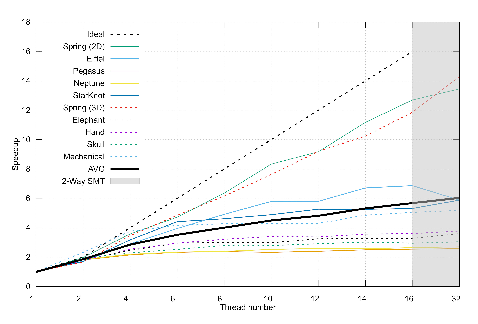
\includegraphics[width=\textwidth]{graph-speedup}
\end{frame*}

\subsection*{Number of tasks}
\begin{frame*}
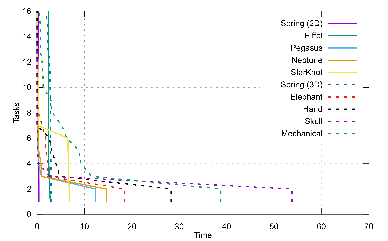
\includegraphics[width=\textwidth]{graph-tasks}
\end{frame*}

\subsection*{Conclusion}
\begin{frame*}
\begin{itemize}
\item Parallel task-based algorithm for computing the augmented Reeb graph.
\item Improved laziness mechanism thank to the locality of growths.
\item Dual sweep for improved parallel performance.
\item OpenMP/\cpluspluslogo{} implementation provided.
\end{itemize}
\begin{block}{What next?}
\begin{itemize}
\item Number of tasks bounded by the number of leaves in the Reeb graph.
\item Number of independent local growths rapidly decreases to $2$.
\end{itemize}
\end{block}
\end{frame*}
\end{document}